\documentclass[a4paper,12]{elsarticle}
\usepackage{amsmath, amsfonts, amssymb, amsthm, bm, graphics, bbm, color}
\usepackage{graphicx}
\usepackage{subfig}
\usepackage{pgfplots}
\usepackage{mathtools}
\usepackage{xcolor,colortbl}
%\usepackage[table]{xcolor}
\usepackage{url}
\usepackage{mathabx}
\usepackage{cancel}
\usepackage{multicol}
\usepackage{float}
\usepackage{caption}
\usepackage{mathalfa}
\usepackage{hyperref}
\usepackage{afterpage}
\usepackage{multirow}
\usepackage{amssymb}
\usepackage{tikz} % Using tikz for line diagrams
\usepackage{lscape} % Using landscape package for large tables.
\usepackage{longtable}
\usepackage{algorithm}
\usepackage{algpseudocode}
\usepackage{listings}
\usepackage{parcolumns}
\usepackage{tikz}

\usetikzlibrary{patterns}

\captionsetup{font=footnotesize}
\captionsetup{width=\textwidth}
\DeclareMathAlphabet\mathbfcal{OMS}{cmsy}{b}{n}
\newtheorem{theorem}{Theorem}[section]
\newtheorem{lemma}[theorem]{Lemma}
\newtheorem{corollary}[theorem]{Corollary}
\newtheorem{proposition}[theorem]{Proposition}
\theoremstyle{definition}
\newtheorem{definition}[theorem]{Definition}
\newtheorem{example}[theorem]{Example}
\newtheorem{remark}[theorem]{Remark}


%center table entries
%\newcolumntype{P}[1]{>{\centering\arraybackslash}p{#1}}


\newcommand\y{\cellcolor{gray!50}}

\newcommand\p{\cellcolor{gray!25}}

\makeatletter
\newcommand\makebig[2]{%
 \@xp\newcommand\@xp*\csname#1\endcsname{\bBigg@{#2}}%
 \@xp\newcommand\@xp*\csname#1l\endcsname{\@xp\mathopen\csname#1\endcsname}%
 \@xp\newcommand\@xp*\csname#1r\endcsname{\@xp\mathclose\csname#1\endcsname}%
}
\makeatother

\makebig{biggg} {3.0}
\makebig{Biggg} {3.5}
\makebig{bigggg}{4.0}
\makebig{Bigggg}{4.5}
\makebig{biggggg}{5.0}
\makebig{Biggggg}{5.5}
\makebig{bigggggg}{6.0}
\makebig{Bigggggg}{6.5}

\newcommand\bovermat[2]{%
 \makebox[0pt][l]{$\smash{\overbrace{\phantom{%
  \begin{matrix}
   #2
  \end{matrix}}}^{\text{#1}}}$}#2}

\newcommand\bundermat[2]{%
 \makebox[0pt][l]{$\smash{\underbrace{\phantom{%
  \begin{matrix}
   #2
  \end{matrix}}}_{\text{#1}}}$}#2}

\newcommand\partialphantom{\vphantom{\frac{\partial e_{P,M}}{\partial w_{1,1}}}}


\newcommand{\raisesym}[2]{\raisebox{0.5\depth}{$#1\Biggggg \}$}}

% redefine paper size
\setlength{\oddsidemargin}{0in}
\setlength{\textwidth}{6.4in}
\setlength{\topmargin}{-0.5in}
\setlength{\textheight}{9.9in}
\setlength{\headheight}{0in}


%slanted vector symbols
\renewcommand{\vec}[1]{\mbox{\boldmath$#1$}}
\newcommand{\vect}[1]{\boldsymbol{#1}}
%vertical d symbol for integrals
\newcommand{\dif}{\mathrm{d}}
\newcommand{\im}{\mathrm{i}}

\newcommand{\Tx}{{\text{Tx}}}
\newcommand{\Rx}{{\text{Rx}}}

\newcommand{\vcE}{{\bm {\mathcal E}}}
\newcommand{\vcH}{{\bm {\mathcal H}}}
\newcommand{\vcJ}{{\bm {\mathcal J}}_0}
\newcommand{\vE}{{\bm {E}}}
\newcommand{\vH}{{\bm {H}}}
\newcommand{\vEb}{{\bm {E}_0}}
\newcommand{\vHb}{{\bm {H}_0}}
\newcommand{\vEa}{{\bm {E}}_\alpha}
\newcommand{\vHa}{{\bm {H}}_\alpha}
\newcommand{\vEd}{{\bm {E}}_\Delta}
\newcommand{\vHd}{{\bm {H}}_\Delta}
\newcommand{\vJ}{{\bm {J}}_0}
\newcommand{\vz}{{\bm {z}}}
\newcommand{\vn}{{\bm {n}}}
\newcommand{\ve}{{\bm {e}}}
\newcommand{\va}{{\bm {a}}}
\newcommand{\vb}{{\bm {b}}}
\newcommand{\vx}{{\bm {x}}}
\newcommand{\vy}{{\bm {y}}}
\newcommand{\vu}{{\bm {u}}}
\newcommand{\vw}{{\bm {w}}}
\newcommand{\vwz}{{\bm {w}}_0}
\newcommand{\vxi}{{\bm {\xi}}}
\newcommand{\vv}{{\bm {v}}}
\newcommand{\vF}{{\bm {F}}}
\newcommand{\vD}{{\bm {D}}}
\newcommand{\vPhi}{{\bm {\Phi}}_0}
\newcommand{\vth}{{\bm {\theta}}}
\newcommand{\vpsi}{{\bm {\psi}}}
\newcommand{\vphi}{{\bm {\phi}}}
\newcommand{\vzero}{{\bm {0}}}
\newcommand{\vX}{{\bm {X}}_\alpha}
\newcommand{\vR}{{\bm {R}}}
\newcommand{\vT}{{\bm {T}}}
\newcommand{\vr}{{\bm {r}}}
\newcommand{\vM}{{\bm {M}}}
\newcommand{\vV}{{\bm {V}}}
\newcommand{\vA}{{\bm {A}}}
\newcommand{\vI}{{\bm {I}}}
\newcommand{\curl}{\nabla \times}


\newcommand{\vvtheta}{{\bm {\vartheta}}}
\newcommand{\vvphi}{{\bm {\varphi}}}
\newcommand{\vtheta}{{\bm {\theta}}}

\DeclareMathOperator*{\esssup}{ess \, sup}
%\pgfplotsset{compat=1.16}
\pgfplotsset{compat=1.15}

\graphicspath{{./Figures/}}


% code snippet style:

\definecolor{codegreen}{rgb}{0,0.6,0}
\definecolor{codegray}{rgb}{0.5,0.5,0.5}
\definecolor{codepurple}{rgb}{0.58,0,0.82}
\definecolor{backcolour}{rgb}{0.95,0.95,0.92}
\lstdefinestyle{mystyle}{
    backgroundcolor=\color{backcolour},   
    commentstyle=\color{codegreen},
    keywordstyle=\color{magenta},
    numberstyle=\tiny\color{codegray},
    stringstyle=\color{codepurple},
    basicstyle=\ttfamily\footnotesize,
    breakatwhitespace=false,         
    breaklines=true,                 
    captionpos=b,                    
    keepspaces=true,                 
    numbers=left,                    
    numbersep=5pt,                  
    showspaces=false,                
    showstringspaces=false,
    showtabs=false,                  
    tabsize=2
}
\lstset{style=mystyle}

\DeclarePairedDelimiter\set\{\}


% Using graphics path, and a flat structure inside the folder, so that we can more easily restructure the project later.
\graphicspath{{./Figures_Elliptic/}}

\begin{document}
% !TeX spellcheck = en_GB

\begin{frontmatter}

\title{Examination of Preconditioners for Simple Magnetostatic Problems}
%
%\author[1]{J. Elgy$^{\rm a*}$\\
%$^{\rm a}$School of Computer Science and Mathematics, Keele University\\
%Keele, Staffordshire U.K\\
%$^*$j.elgy@keele.ac.uk}
\cortext[cor1]{*}
\affiliation[1]{organization={School of Computer Science and Mathematics, Keele University},
city={Keele, Staffordshire},
country={UK}}
 
\author[1]{J. Elgy\corref{cor1}} \ead{j.elgy@keele.ac.uk}

%\maketitle

\begin{abstract}

\end{abstract}

\begin{keyword} 
\end{keyword}

\end{frontmatter}

\section{Introduction}\label{sect:intro}

\subsection{Model Problem}
%\begin{equation}\label{eqn:system}
%\begin{alignedat}{2}
%\curl \curl \boldsymbol{G} + \boldsymbol{G} &= \boldsymbol{F} &&\quad \text{in } \Omega \in \mathbb{R}^3 \\
%\boldsymbol{n} \times \boldsymbol{G} &= \boldsymbol{n} \times \boldsymbol{G}^{(exact)} &&\quad \text{on } \Gamma = \partial \Omega
%\end{alignedat}
%\end{equation}
%%
%For a simple divergence free elliptic model problem where $\boldsymbol{G}^{(exact)} = [\mathrm{sin}(y), 0, 0]$ we have the right hand side $\boldsymbol{F} = [2\mathrm{sin}(y), 0, 0]$. 
%
%For the standard $\boldsymbol{H}(\rm{curl})$ conforming finite element space \cite{Monk2017} the weak form of this problem is: Find $\boldsymbol{u} \in \boldsymbol{H}_D(\rm{curl})$ such that
%\begin{equation}\label{eqn:weak_form}
%\int_\Omega \curl \vec{u} \, \curl \vec{v} \,\mathrm{d}\Omega + \int_\Omega \vec{u}\vec{v} \,\mathrm{d}\Omega = \int_\Omega \boldsymbol{F}\vec{v} \, \mathrm{d}\Omega,
%\end{equation}
for all $\vec{v} \in \boldsymbol{H}_0(\rm{curl})$ and $k^2 = |\vec{k}|^2 > 0$ being homogeneous and isotropic in $\Omega$. Here, $\boldsymbol{H}(\rm{curl})$ is the high order space defined by
\begin{equation*}
\boldsymbol{H}(\rm{curl}) := \left\{ \vec{a} \in L^2(\Omega)^3 | \curl \vec{a} \in L^2(\Omega)^3\right\},
\end{equation*}
where $L^2(\Omega)$ denotes the space of square integrable functions. Considering Dirichlet boundary conditions and setting $\vec{v}$ to vanish on the boundary, the appropriate subspaces for this problem are
\begin{equation*}
\begin{alignedat}{2}
\boldsymbol{H}_D(\rm{curl}) &:= \left\{ \vec{a} \in \vec{H}(\rm{curl}) | \vec{n}\times \vec{a} = \vec{n} \times \vec{E}^{(exact)} \text{ on } \Gamma\right\}\\
\boldsymbol{H}_0(\rm{curl}) &:= \left\{ \vec{a} \in \vec{H}(\rm{curl}) | \vec{n}\times \vec{a} = \vec{0} \text{ on } \Gamma\right\}.
\end{alignedat}
\end{equation*}

The Galerkin finite element discretisation of the variational statement (\ref{eqn:weak_form}) is the large linear system
\begin{equation}\label{eqn:lse}
\mathbf{A}\mathbf{q} = \mathbf{r}
\end{equation}
where $\mathbf{A}$ is a large sparse matrix of size $N_d$. The symmetric sparse matrix $\mathbf{A}$ is indefinite, and consequently may be difficult to solve.

\textcolor{cyan}{Should expand, mostly here to have something to cross reference.}


\section{Preconditioners}
Three different preconditioners are considered, The Local (Jacobi) preconditioner, the Balancing Domain Decomposition with Constraints (BDDC) preconditioner, and a geometric Multigrid preconditioner.

\subsection{Local Preconditioner}
The Local preconditioner, as implemented in \texttt{NGSolve}, is a simple Jacobi preconditioner. For this preconditioner, the preconditioner matrix $\mathbf{P}$ is chosen as $\mathbf{P} := \mathrm{diag}(\mathbf{A})$. Using Static condensation, the system matrix $\mathbf{A}$ can be partitioned into local $L$ and interface $E$ degrees of freedom as 
%
\begin{equation*}
\mathbf{A} = \begin{bmatrix}
\mathbf{A}_{LL} & \mathbf{A}_{LE} \\ \mathbf{A}_{EL} & \mathbf{A}_{EE}
\end{bmatrix},
\end{equation*}
%
where internal degrees of freedom are eliminated via the Schur Complement~\cite{Guyan1965} 
\begin{equation*}
\mathbf{S} = \mathbf{A}_{EE} - \mathbf{A}_{EL} \mathbf{A}_{LL}^{-1} \mathbf{A}_{LE}.
\end{equation*}
%
When assembling the bilinear form for use with static condensation, \texttt{NGSolve} computes $\mathbf{S}$, thus
%
\begin{equation*}
\mathbf{A} = \begin{bmatrix}
0 &0 \\ 0 & \mathbf{S}
\end{bmatrix},
\end{equation*}
%
and the preconditioner corresponds to
\begin{equation*}
\mathbf{P} = \begin{bmatrix}
0 &0 \\ 0 & \mathrm{diag}(\mathbf{S})
\end{bmatrix}.
\end{equation*}

\subsection{Multigrid Preconditioner}
The multigrid preconditioner implemented by \texttt{NGSolve} uses a sequence of successively refined meshes such that a direct solve for the coarsest mesh is possible. Block Gauss-Seidel smoothers are then employed for finer meshes.

1 V cycle
Uses vertex patch for complex FES smoothing

For the linear system (\ref{eqn:lse}), the multigrid preconditioner
\begin{algorithm}
\caption{Multigrid preconditioner $\mathbf{P}^{-1}_{l} : \vec{r} \rightarrow \vec{q}$}
\begin{algorithmic}
\For {$0 \le l \le L$}
\If{$l > 0$}
\State $\vec{q} \gets \vec{0}$
\State $\vec{q} \gets \vec{w} + \mathbf{P_l}$
\Else
\State $\vec{q} \gets \mathbf{A}_0^{-1} \vec{r}$
\EndIf
\EndFor


\end{algorithmic}
\end{algorithm}





\section{Software}\label{sect:software}
The  computational resources were used to perform the simulations in this paper correspond to  workstations with the following specifications: Intel i7-9700K CPU with a clock speed of 3.60GHz with 64GB DDR4 RAM.

The software used for this work \texttt{NGSolve} (version 6.2.2302) and \texttt{Netgen} (version 6.2.2302)~\cite{NGSolve,zaglmayrphd,netgendet}, \texttt{SciPy}~\cite{2020SciPy-NMeth} (version 1.10.1), \texttt{NumPy} (version 1.24.2)~\cite{harris2020array}.


\section{Results}\label{sect:results}
Example of a unit radius sphere formed on a sequence of meshes, $m_0, m_1, m_2$, where the subscript refers to the levels of refinement. Elements are flagged for refinement only inside, and on the surface of, the sphere. The sphere is discretised using 12\,198, 58\,965, and 247\,952 unstructured tetrahedral elements with $p=2$. The following comparison (Figures~\ref{fig:mem_usage_breakdown} and~\ref{fig:mem_usage_comparison}) compares the computation time and memory usage of the local, BDDC, and multigrid preconditioners on the finest mesh. The figures show that, in this example, the Multigrid preconditioner is slightly faster and requires less memory than the BDDC or Local preconditioners, although, from Figure~\ref{fig:mem_usage_breakdown}, we observe that the removal of the gradient terms, which involves the inverse of a matrix formed on the finest grid, and the computation of the errors contributes a majority of the time taken. The performance benefits associated with the Multigrid preconditioner are explained by the faster construction of the preconditioner.

\begin{figure}[h!]
\centering
$
\begin{array}{c c c}
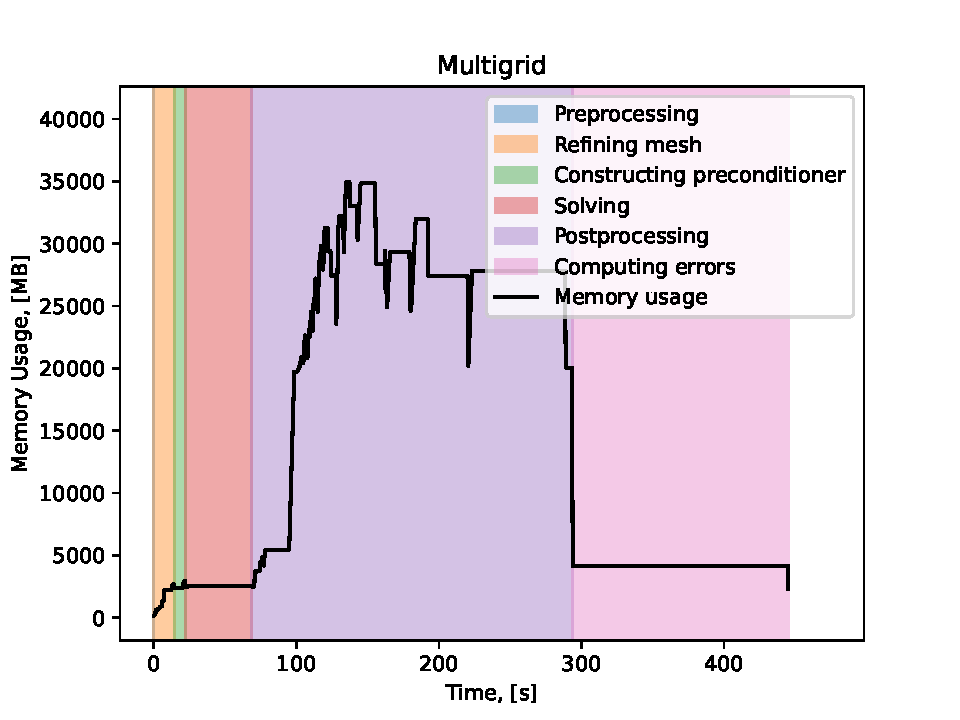
\includegraphics[width=0.3\textwidth]{Sphere_p=2_mem_usage_Multigrid} & 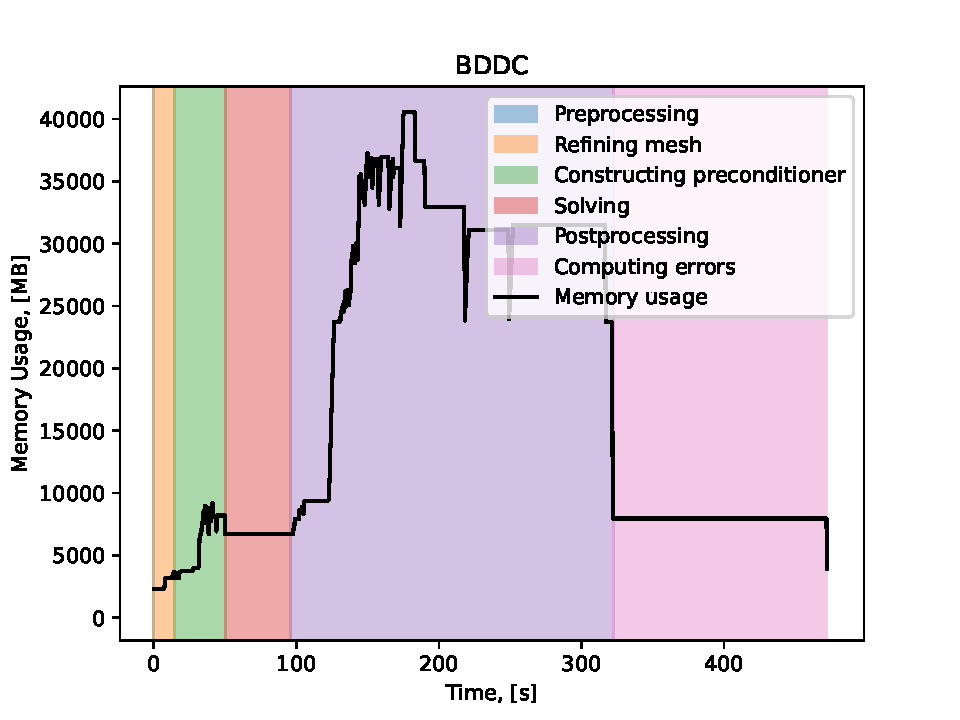
\includegraphics[width=0.3\textwidth]{Sphere_p=2_mem_usage_BDDC} & 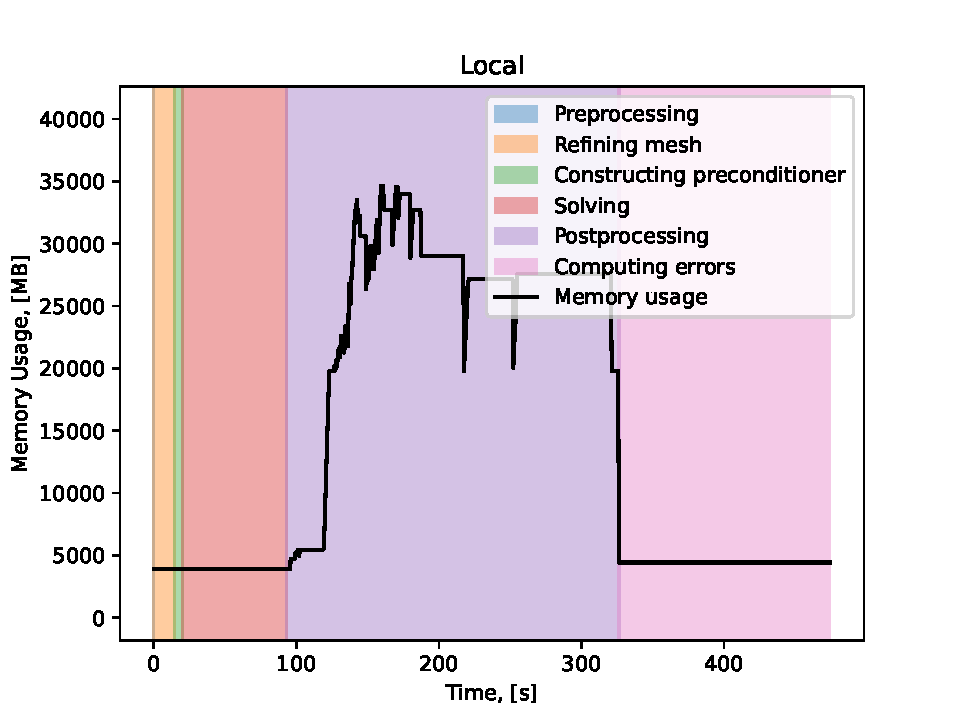
\includegraphics[width=0.3\textwidth]{Sphere_p=2_mem_usage_Local} \\
(a) & (b) & (c)
\end{array}
$
\caption{Magnetic sphere with unit radius and $\mu_r = 20$ discretised using $p=2$ and a sequence of meshes with 12\,198, 58\,965, and 247\,952 unstructured tetrahedra. Figure shows memory usage and computation time when considering (($a$) BDDC, ($b$) Multigrid, and ($c$) local preconditioners. }
\label{fig:mem_usage_breakdown}
\end{figure}

\begin{figure}[h!]
\centering
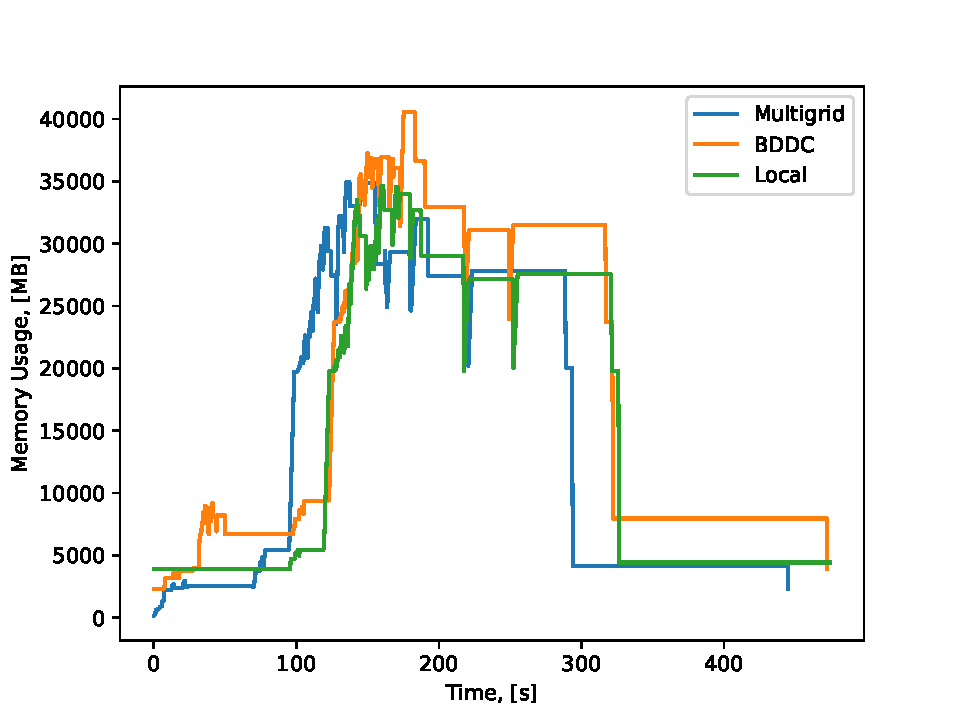
\includegraphics[width=0.45\textwidth]{Sphere_p=2_mem_usage}
\caption{Magnetic sphere with unit radius and $\mu_r = 20$ discretised using $p=2$ and a sequence of meshes with 12\,198, 58\,965, and 247\,952 unstructured tetrahedra. Figure shows memory usage and computation time when considering each preconditioner. }
\label{fig:mem_usage_comparison}
\end{figure}

Given that the postprocessing and construction of the projection operator is independent of the preconditioner, and requires similar computational resources in all 3 examples, future examples will not include this step with the understanding that the error in the curl of $\mathbf{A}$ is unaffected, i.e. the curl of a gradient is zero. With similar reasoning, the time required to compute the error is also constant.

\bibliographystyle{acm}
\bibliography{paperbib}

\end{document}
